\documentclass{standalone}
\usepackage{tikz}
\usetikzlibrary{patterns, positioning}


\begin{document}
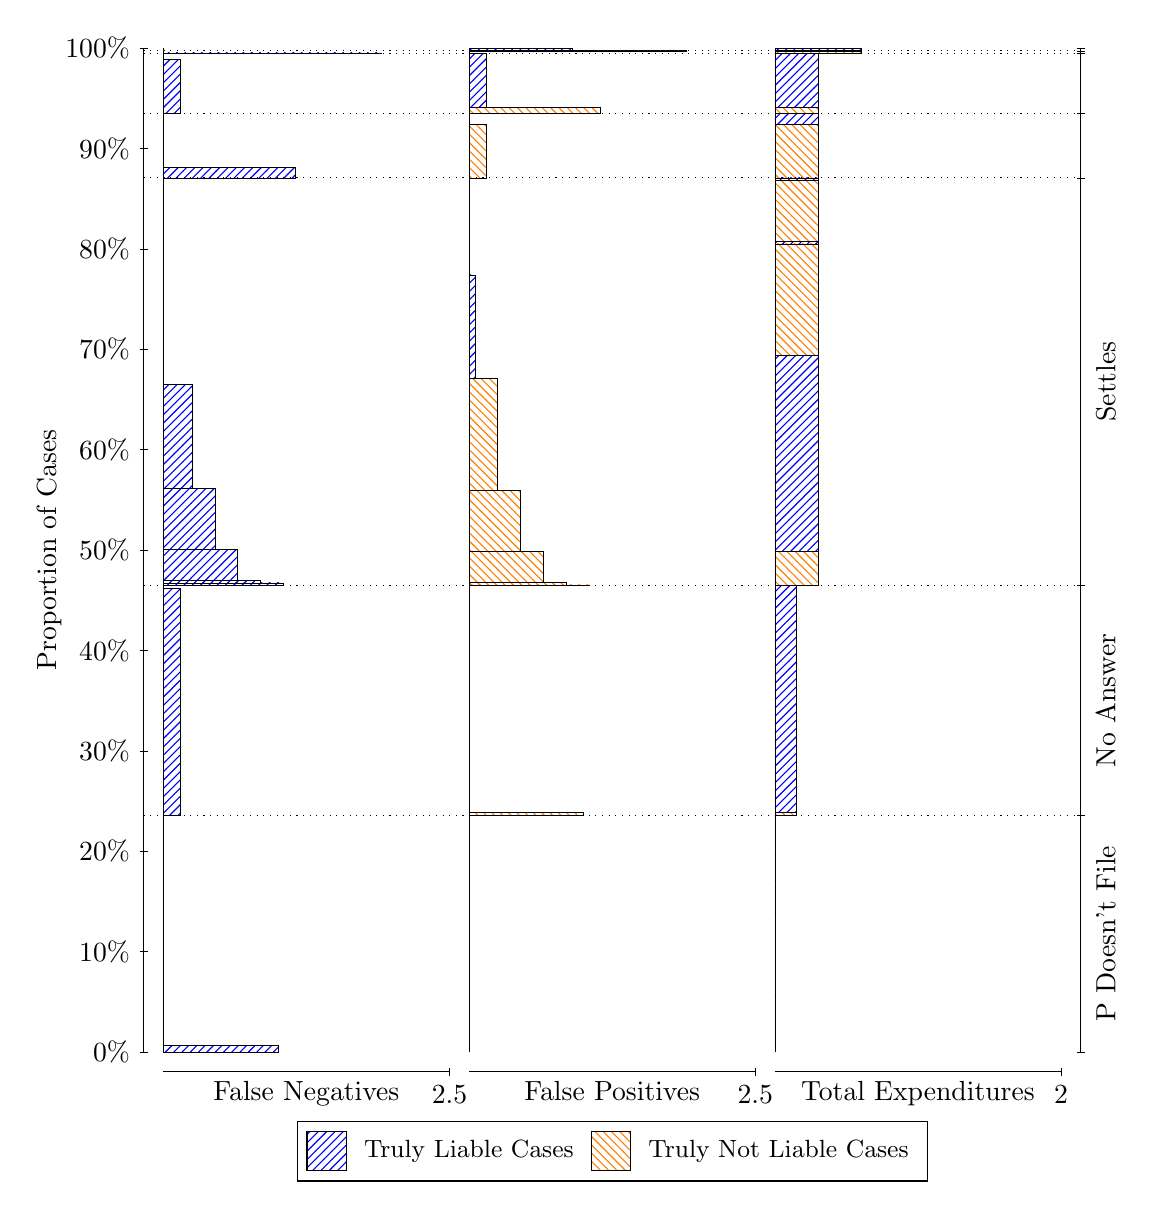
\begin{tikzpicture}
\draw[black, very thin] (1.5,1.75) -- (1.5,14.5);
\node[rotate=90, text=black, anchor=center] at (0.3, 8.125) {Proportion of Cases};
\draw[black, very thin] (1.45,1.75) -- (1.55,1.75);
\node[text=black, anchor=east] at (1.45, 1.75) {0\%};
\draw[black, very thin] (1.45,3.025) -- (1.55,3.025);
\node[text=black, anchor=east] at (1.45, 3.025) {10\%};
\draw[black, very thin] (1.45,4.3) -- (1.55,4.3);
\node[text=black, anchor=east] at (1.45, 4.3) {20\%};
\draw[black, very thin] (1.45,5.575) -- (1.55,5.575);
\node[text=black, anchor=east] at (1.45, 5.575) {30\%};
\draw[black, very thin] (1.45,6.85) -- (1.55,6.85);
\node[text=black, anchor=east] at (1.45, 6.85) {40\%};
\draw[black, very thin] (1.45,8.125) -- (1.55,8.125);
\node[text=black, anchor=east] at (1.45, 8.125) {50\%};
\draw[black, very thin] (1.45,9.4) -- (1.55,9.4);
\node[text=black, anchor=east] at (1.45, 9.4) {60\%};
\draw[black, very thin] (1.45,10.675) -- (1.55,10.675);
\node[text=black, anchor=east] at (1.45, 10.675) {70\%};
\draw[black, very thin] (1.45,11.95) -- (1.55,11.95);
\node[text=black, anchor=east] at (1.45, 11.95) {80\%};
\draw[black, very thin] (1.45,13.225) -- (1.55,13.225);
\node[text=black, anchor=east] at (1.45, 13.225) {90\%};
\draw[black, very thin] (1.45,14.5) -- (1.55,14.5);
\node[text=black, anchor=east] at (1.45, 14.5) {100\%};

\draw[black, very thin] (13.4,1.75) -- (13.4,14.5);
\draw[black, very thin] (13.35,1.75) -- (13.45,1.75);
\node[anchor=west] at (13.35, 1.75) {};
\draw[black, very thin] (13.35,4.7537) -- (13.45,4.7537);
\node[anchor=west] at (13.35, 4.7537) {};
\draw[black, very thin] (13.35,7.675) -- (13.45,7.675);
\node[anchor=west] at (13.35, 7.675) {};
\draw[black, very thin] (13.35,12.852) -- (13.45,12.852);
\node[anchor=west] at (13.35, 12.852) {};
\draw[black, very thin] (13.35,13.666) -- (13.45,13.666);
\node[anchor=west] at (13.35, 13.666) {};
\draw[black, very thin] (13.35,14.433) -- (13.45,14.433);
\node[anchor=west] at (13.35, 14.433) {};
\draw[black, very thin] (13.35,14.463) -- (13.45,14.463);
\node[anchor=west] at (13.35, 14.463) {};
\draw[black, very thin] (13.35,14.5) -- (13.45,14.5);
\node[anchor=west] at (13.35, 14.5) {};

\draw[black, very thin, pattern color=blue, pattern=north east lines] (1.75,1.75) rectangle (3.2033,1.8313);
\draw[black, very thin, pattern color=orange, pattern=north west lines] (1.75,1.8313) rectangle (1.75,4.7537);
\draw[black, very thin, pattern color=blue, pattern=north east lines] (1.75,4.7537) rectangle (1.968,7.6345);
\draw[black, very thin, pattern color=orange, pattern=north west lines] (1.75,7.6345) rectangle (1.75,7.675);
\draw[black, very thin, pattern color=blue, pattern=north east lines] (1.75,7.675) rectangle (3.276,7.7077);
\draw[black, very thin, pattern color=blue, pattern=north east lines] (1.75,7.7077) rectangle (2.9853,7.7405);
\draw[black, very thin, pattern color=blue, pattern=north east lines] (1.75,7.7405) rectangle (2.6947,8.1353);
\draw[black, very thin, pattern color=blue, pattern=north east lines] (1.75,8.1353) rectangle (2.404,8.9087);
\draw[black, very thin, pattern color=blue, pattern=north east lines] (1.75,8.9087) rectangle (2.1133,10.225);
\draw[black, very thin, pattern color=orange, pattern=north west lines] (1.75,10.225) rectangle (1.75,12.852);
\draw[black, very thin, pattern color=blue, pattern=north east lines] (1.75,12.852) rectangle (3.4213,12.987);
\draw[black, very thin, pattern color=orange, pattern=north west lines] (1.75,12.987) rectangle (1.75,13.666);
\draw[black, very thin, pattern color=blue, pattern=north east lines] (1.75,13.666) rectangle (1.968,14.357);
\draw[black, very thin, pattern color=orange, pattern=north west lines] (1.75,14.357) rectangle (1.75,14.433);
\draw[black, very thin, pattern color=blue, pattern=north east lines] (1.75,14.433) rectangle (4.5113,14.438);
\draw[black, very thin, pattern color=orange, pattern=north west lines] (1.75,14.438) rectangle (1.75,14.463);
\draw[black, very thin, pattern color=orange, pattern=north west lines] (1.75,14.463) rectangle (1.75,14.467);
\draw[black, very thin, pattern color=blue, pattern=north east lines] (1.75,14.467) rectangle (1.75,14.5);
\draw[black, very thin, pattern color=orange, pattern=north west lines] (5.6333,1.75) rectangle (5.6333,4.6724);
\draw[black, very thin, pattern color=blue, pattern=north east lines] (5.6333,4.6724) rectangle (5.6333,4.7537);
\draw[black, very thin, pattern color=orange, pattern=north west lines] (5.6333,4.7537) rectangle (7.0867,4.7942);
\draw[black, very thin, pattern color=blue, pattern=north east lines] (5.6333,4.7942) rectangle (5.6333,7.675);
\draw[black, very thin, pattern color=orange, pattern=north west lines] (5.6333,7.675) rectangle (7.1593,7.6811);
\draw[black, very thin, pattern color=orange, pattern=north west lines] (5.6333,7.6811) rectangle (6.8687,7.714);
\draw[black, very thin, pattern color=orange, pattern=north west lines] (5.6333,7.714) rectangle (6.578,8.1087);
\draw[black, very thin, pattern color=orange, pattern=north west lines] (5.6333,8.1087) rectangle (6.2873,8.8819);
\draw[black, very thin, pattern color=orange, pattern=north west lines] (5.6333,8.8819) rectangle (5.9967,10.302);
\draw[black, very thin, pattern color=blue, pattern=north east lines] (5.6333,10.302) rectangle (5.706,11.619);
\draw[black, very thin, pattern color=blue, pattern=north east lines] (5.6333,11.619) rectangle (5.6333,12.852);
\draw[black, very thin, pattern color=orange, pattern=north west lines] (5.6333,12.852) rectangle (5.8513,13.532);
\draw[black, very thin, pattern color=blue, pattern=north east lines] (5.6333,13.532) rectangle (5.6333,13.666);
\draw[black, very thin, pattern color=orange, pattern=north west lines] (5.6333,13.666) rectangle (7.3047,13.743);
\draw[black, very thin, pattern color=blue, pattern=north east lines] (5.6333,13.743) rectangle (5.8513,14.433);
\draw[black, very thin, pattern color=orange, pattern=north west lines] (5.6333,14.433) rectangle (5.6333,14.457);
\draw[black, very thin, pattern color=blue, pattern=north east lines] (5.6333,14.457) rectangle (5.6333,14.463);
\draw[black, very thin, pattern color=orange, pattern=north west lines] (5.6333,14.463) rectangle (8.3947,14.467);
\draw[black, very thin, pattern color=blue, pattern=north east lines] (5.6333,14.467) rectangle (6.9413,14.5);
\draw[black, very thin, pattern color=orange, pattern=north west lines] (9.5167,1.75) rectangle (9.5167,4.6724);
\draw[black, very thin, pattern color=blue, pattern=north east lines] (9.5167,4.6724) rectangle (9.5167,4.7537);
\draw[black, very thin, pattern color=orange, pattern=north west lines] (9.5167,4.7537) rectangle (9.7892,4.7942);
\draw[black, very thin, pattern color=blue, pattern=north east lines] (9.5167,4.7942) rectangle (9.7892,7.675);
\draw[black, very thin, pattern color=orange, pattern=north west lines] (9.5167,7.675) rectangle (10.062,8.1087);
\draw[black, very thin, pattern color=blue, pattern=north east lines] (9.5167,8.1087) rectangle (10.062,10.593);
\draw[black, very thin, pattern color=orange, pattern=north west lines] (9.5167,10.593) rectangle (10.062,12.014);
\draw[black, very thin, pattern color=blue, pattern=north east lines] (9.5167,12.014) rectangle (10.062,12.046);
\draw[black, very thin, pattern color=orange, pattern=north west lines] (9.5167,12.046) rectangle (10.062,12.82);
\draw[black, very thin, pattern color=blue, pattern=north east lines] (9.5167,12.82) rectangle (10.062,12.852);
\draw[black, very thin, pattern color=orange, pattern=north west lines] (9.5167,12.852) rectangle (10.062,13.532);
\draw[black, very thin, pattern color=blue, pattern=north east lines] (9.5167,13.532) rectangle (10.062,13.666);
\draw[black, very thin, pattern color=orange, pattern=north west lines] (9.5167,13.666) rectangle (10.062,13.743);
\draw[black, very thin, pattern color=blue, pattern=north east lines] (9.5167,13.743) rectangle (10.062,14.433);
\draw[black, very thin, pattern color=orange, pattern=north west lines] (9.5167,14.433) rectangle (10.607,14.457);
\draw[black, very thin, pattern color=blue, pattern=north east lines] (9.5167,14.457) rectangle (10.607,14.463);
\draw[black, very thin, pattern color=orange, pattern=north west lines] (9.5167,14.463) rectangle (10.607,14.467);
\draw[black, very thin, pattern color=blue, pattern=north east lines] (9.5167,14.467) rectangle (10.607,14.5);
\draw[black, dotted] (1.5,4.7537) -- (13.4,4.7537);
\draw[black, dotted] (1.5,7.675) -- (13.4,7.675);
\draw[black, dotted] (1.5,12.852) -- (13.4,12.852);
\draw[black, dotted] (1.5,13.666) -- (13.4,13.666);
\draw[black, dotted] (1.5,14.433) -- (13.4,14.433);
\draw[black, dotted] (1.5,14.463) -- (13.4,14.463);
\draw[black, very thin] (1.75,1.5) -- (5.3833,1.5);
\node[text=black, anchor=north] at (3.5667, 1.5) {False Negatives};
\draw[black, very thin] (5.3833,1.45) -- (5.3833,1.55);
\node[text=black, anchor=north] at (5.3833, 1.45) {2.5};

\draw[black, very thin] (5.6333,1.5) -- (9.2667,1.5);
\node[text=black, anchor=north] at (7.45, 1.5) {False Positives};
\draw[black, very thin] (9.2667,1.45) -- (9.2667,1.55);
\node[text=black, anchor=north] at (9.2667, 1.45) {2.5};

\draw[black, very thin] (9.5167,1.5) -- (13.15,1.5);
\node[text=black, anchor=north] at (11.333, 1.5) {Total Expenditures};
\draw[black, very thin] (13.15,1.45) -- (13.15,1.55);
\node[text=black, anchor=north] at (13.15, 1.45) {2};

\node[text=black, centered, rotate=90] at (13.72, 3.2518) {P Doesn't File};
\node[text=black, centered, rotate=90] at (13.72, 6.2143) {No Answer};
\node[text=black, centered, rotate=90] at (13.72, 10.264) {Settles};





\draw (7.449999999999999,1.5) node[draw=none] (baseCoordinate) {};
\begin{scope}[align=center]
        \matrix[scale=0.5, draw=black, below=0.5cm of baseCoordinate, nodes={draw}, column sep=0.1cm]{
            \node[rectangle, draw, minimum width=0.5cm, minimum height=0.5cm, pattern color=blue, pattern=north east lines] {}; &
            \node[draw=none, font=\small, text=black] (B) {Truly Liable Cases}; &
            \node[rectangle, draw, minimum width=0.5cm, minimum height=0.5cm, pattern color=orange, pattern=north west lines] {}; &
            \node[draw=none, font=\small, text=black] (B) {Truly Not Liable Cases}; \\
            };
\end{scope}

\end{tikzpicture}
\end{document}